\documentclass[11pt,letterpaper]{article}
\usepackage[lmargin=1in,rmargin=1in,tmargin=1in,bmargin=1in]{geometry}
\usepackage{../style/homework}
\usepackage{../style/commands}
\setbool{quotetype}{false} % True: Side; False: Under
\setbool{hideans}{true} % Student: True; Instructor: False

% -------------------
% Content
% -------------------
\begin{document}

\homework{7: Due 06/07}{Science is simply common sense at its best, that is, rigidly accurate in observation, and merciless to fallacy in logic.}{Thomas Huxley}

% Problem 1
\problem{10} Plot the quadratic function $y= 4 - (x + 6)^2$ as accurately as possible. Your sketch should include the vertex and axis of symmetry. 
	\[
	\fbox{
	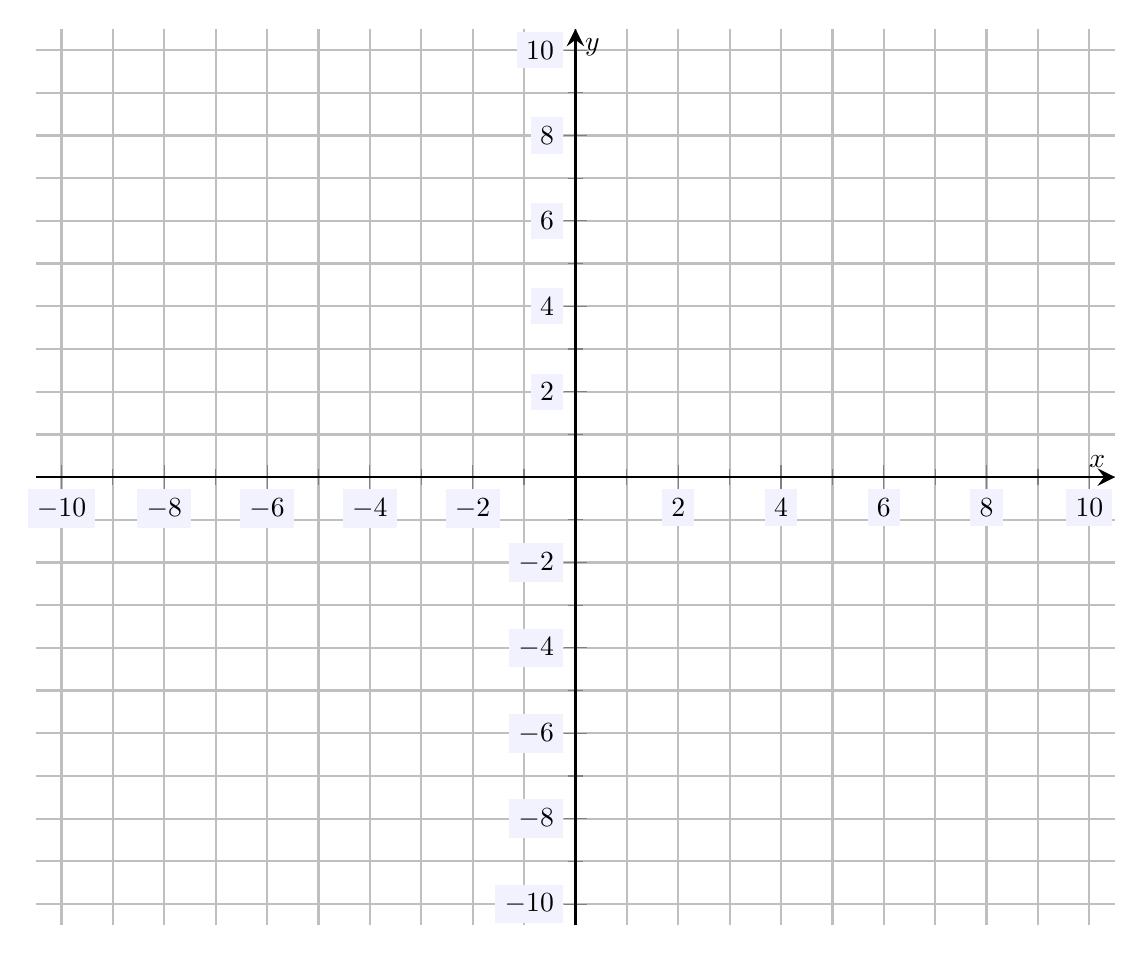
\begin{tikzpicture}[scale=2,every node/.style={scale=0.5}]
	\begin{axis}[
	grid=both,
	axis lines=middle,
	ticklabel style={fill=blue!5!white},
	xmin= -10.5, xmax=10.5,
	ymin= -10.5, ymax=10.5,
	xtick={-10,-8,-6,-4,-2,0,2,4,6,8,10},
	ytick={-10,-8,-6,-4,-2,0,2,4,6,8,10},
	minor tick = {-10,-9,...,10},
	xlabel=\(x\),ylabel=\(y\),
	]
	\end{axis}
	\end{tikzpicture}
	}
	\] 



\newpage



% Problem 2
\problem{10} Find the vertex form of $f(x)= x^2 - 12x + 41$. Also, find the vertex and axis of symmetry of $f(x)$. 



\newpage



% Problem 3
\problem{10} Find the vertex and axis of symmetry of $g(x)= -3x^2 + 24x - 37$. 



\newpage



% Problem 4
\problem{10} Consider the quadratic function $h(x)= 4x^2 - 12x + 6$.
        \begin{enumerate}[(a)]
        \item Determine if the parabola opens upwards or downwards.
        \item Is the parabola convex or concave?
        \item Does the parabola have a maximum or minimum? 
        \item Find the vertex and axis of symmetry. 
        \item Find the maximum/minimum value of $h(x)$. 
        \end{enumerate}



\newpage



% Problem 5
\problem{10} Consider the quadratic function $j(x)= -x^2 - 4x + 1$.
        \begin{enumerate}[(a)]
        \item Determine if the parabola opens upwards or downwards.
        \item Is the parabola convex or concave?
        \item Does the parabola have a maximum or minimum? 
        \item Find the vertex and axis of symmetry. 
        \item Find the maximum/minimum value of $j(x)$. 
        \end{enumerate}



\newpage



% Problem 6
\problem{10} Factor the following:
	\begin{enumerate}[(a)]
	\item $x^2 - 64$
	\item $4x - 20x^2$
	\item $9x^2 - 25$
	\item $5x^2 + 60x$
	\end{enumerate}



\newpage



% Problem 7
\problem{10} Factor the following completely: $4x^2 + 20x - 24$



\newpage



% Problem 8
\problem{10} Use completing the square to solve the following equation:
	\[
	4x^2= 16x - 24
	\]



\newpage



% Problem 9
\problem{10} Solve the following quadratic equation by factoring:
	\[
	10x= 24 - x^2
	\]



\newpage



% Problem 10
\problem{10} Solve the following quadratic equation:
	\[
	x(10 - x)= 25
	\]


\end{document}